\section{Dataset Deep Dive}
We conducted a systematic descriptive analysis of the released training split to quantify its distributional, linguistic, and structural properties.
Our analysis reveals several key characteristics regarding its scale, multi-label nature, class imbalance, and co-occurrence structure, which collectively motivate our architectural design choices.

\textbf{Scale and Multilinguality.} The corpus contains 1,699 documents in five languages: Bulgarian (BG), Portuguese (PT), English (EN), Hindi (HI), and Russian (RU). The distribution is relatively balanced across Bulgarian, Portuguese, and English (\(\approx\) 399--401 documents each), with 366 Hindi documents and 133 Russian documents. This multilingual context is critical for assessing the cross-lingual generalization capabilities of classification models.

\textbf{Multi-Label Nature.} Building upon this multilingual foundation, a defining feature of the dataset is the high frequency of multi-label annotations. A majority of documents (54.0\%) are assigned more than one narrative, with an average of 2.28 narrative labels per document and a maximum of 8. This observation confirms that multi-label modeling is essential; treating the task as a series of independent single-label classifications would discard significant structural information present in the data.

\textbf{Label Frequency and Extreme Imbalance.} The complexity of the multi-label structure is further compounded by severe class imbalance. The taxonomy consists of 22 distinct narrative labels and 95 sub-narrative labels, distributed in a strongly skewed manner. The most frequent narrative appears 584 times (representing \(\approx\) 15.1\% of all narrative annotations in the multilingual training set), while the least frequent occurs only 9 times. This yields an imbalance ratio of approximately 65:1, creating a classic long-tailed distribution. Notably, the dataset also includes a generic Other category for documents that do not fit any predefined narrative, which accounts for a substantial portion of the data and requires models to learn a negative class boundary against all defined narratives. The most prevalent narratives are dominated by war-related topics (e.g., `URW: Discrediting Ukraine`, `URW: Discrediting the West, Diplomacy`), highlighting the dataset's focus on high-stakes domains. This sparsity poses a significant challenge for supervised models, which can become biased towards majority classes and fail to generalize to rare but meaningful narratives.

\begin{figure}[ht]
  \centering
  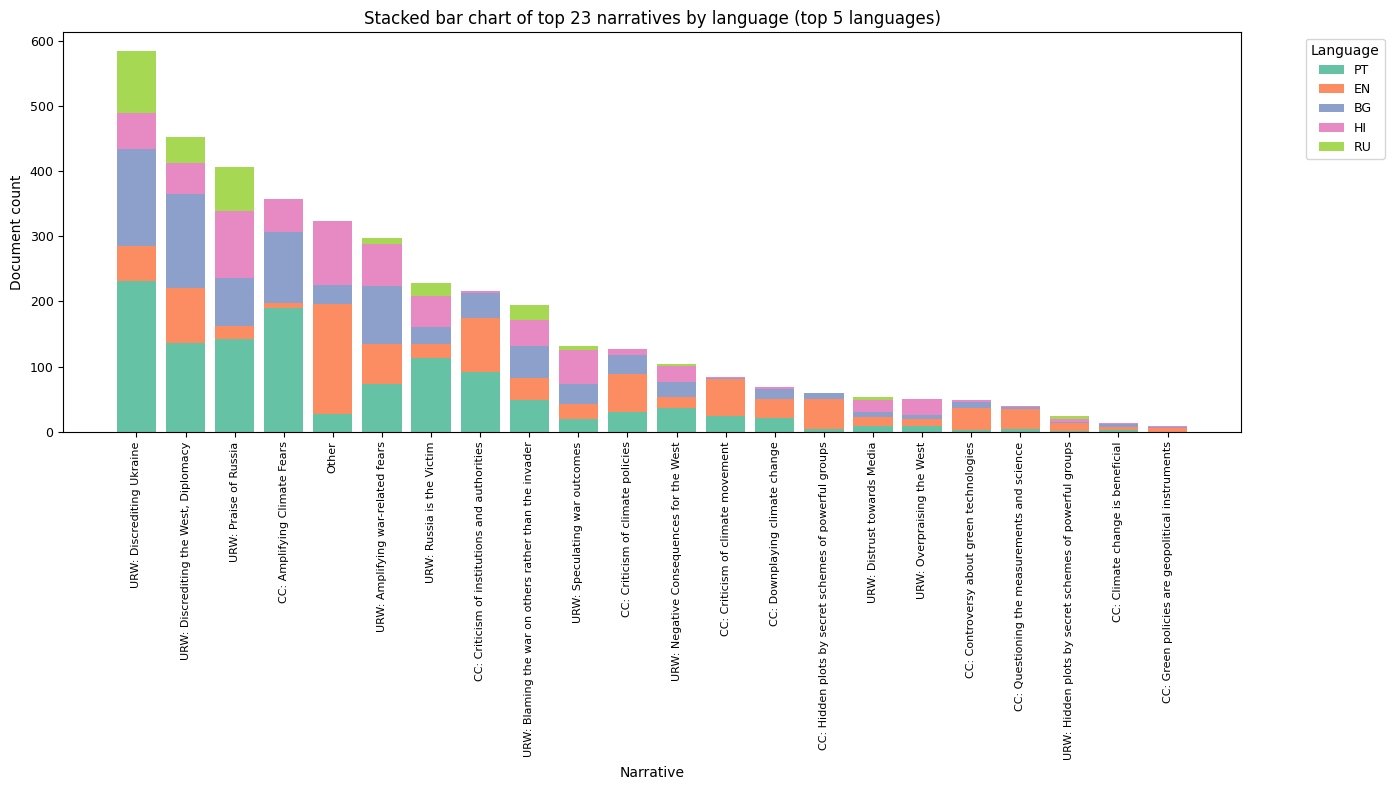
\includegraphics[width=1\linewidth]{images/data_description/narrative_distribution.png}
  \caption{Long-tailed distribution of narrative labels in the SemEval-2025 training set. The bar chart shows the frequency of each coarse narrative, illustrating that a small number of narratives account for a large fraction of annotations while many narratives have very few examples. This severe imbalance motivates the use of zero-shot and evidence-grounded LLM approaches that do not rely on large per-class training counts.}
  \label{fig:narrative_distribution}
\end{figure}

\textbf{Structured Label Co-occurrence.} Despite this imbalance, the relationships between labels are not random but exhibit meaningful patterns. Co-occurrence analysis reveals that while most pairs of narratives rarely appear together, certain thematically-linked pairs exhibit strong associations. For example, documents often combine \emph{attack} and \emph{counter-attack} narratives (e.g., discrediting Ukraine together with discrediting the West), or pair attacks on an adversary with \emph{praise of allies} (e.g., discrediting Ukraine alongside praise of Russia). Other recurrent patterns reflect causal framing, such as linking sanctions to economic hardship, or pairings between diplomatic failure and critiques of legitimacy. Military operations are frequently co-annotated with victim/threat framings, and conspiracy claims commonly appear together with explicit attribution to external actors. These recurring narrative couplings illustrate that co-occurrence captures structured discourse strategies in which labels reinforce one another. More advanced analysis further reveals directional dependencies (i.e., \(P(B\mid A) eq P(A\mid B)\)).

% Combined co-occurrence visualizations (two panels)
\begin{figure}[ht]
  \centering
  \begin{minipage}[b]{0.49\linewidth}
    \centering
  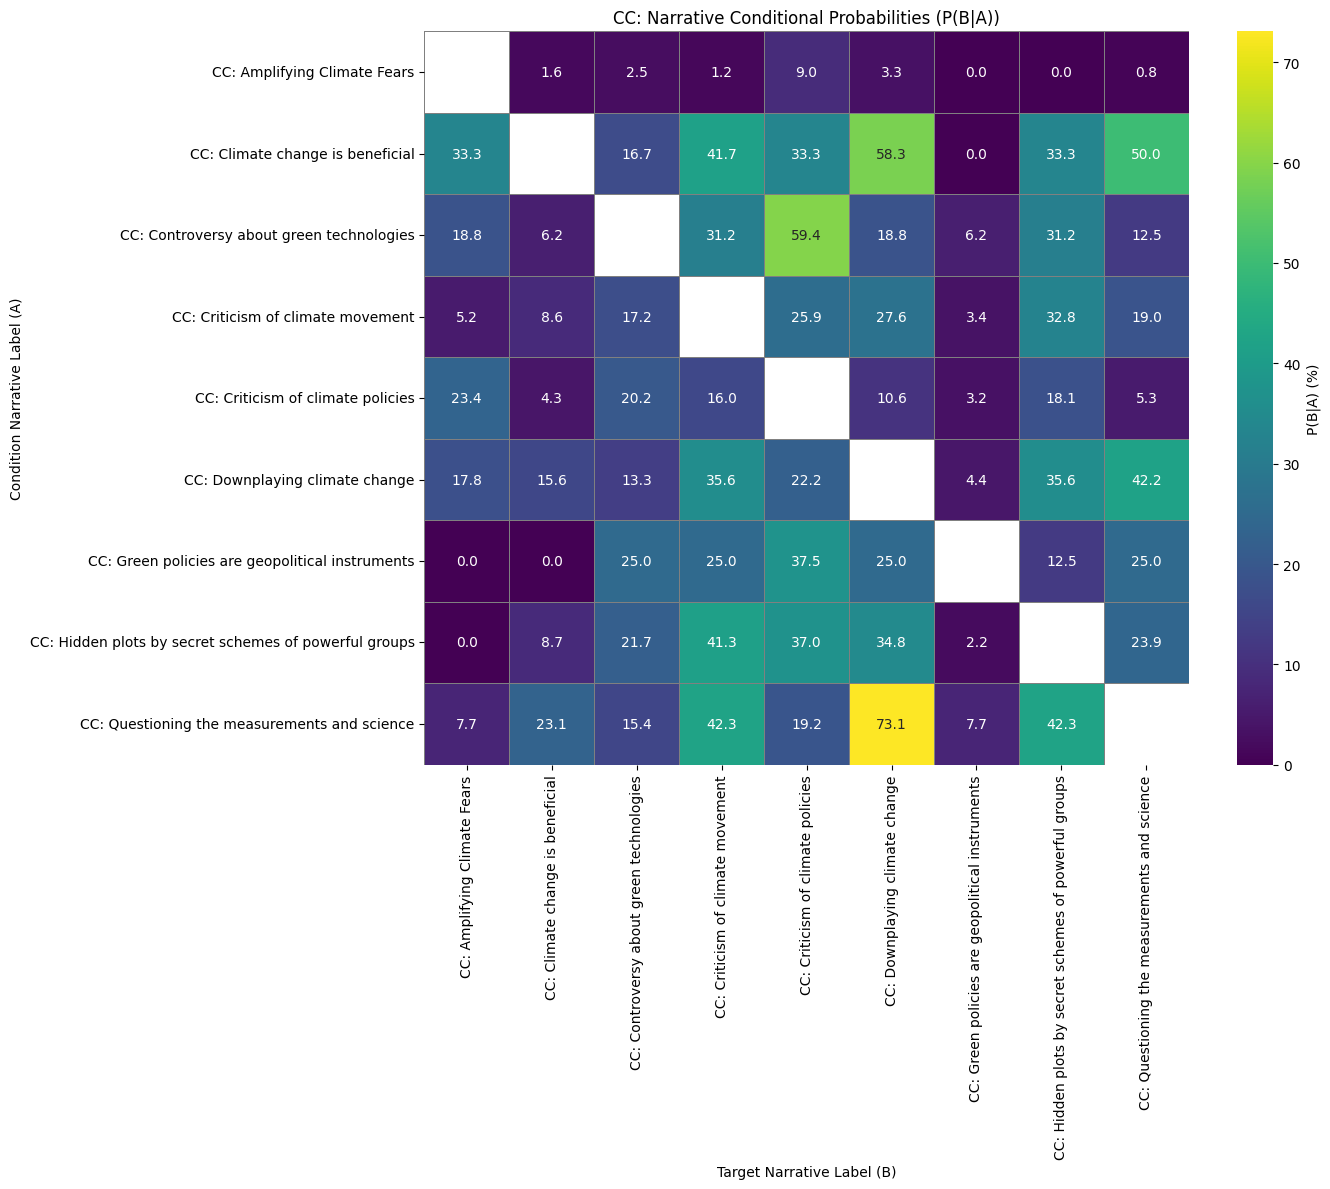
\includegraphics[width=\linewidth]{images/CC_narratives_conditional_probability.png}
  \par\medskip\centering\footnotesize (a) CC narratives heatmap\par
  \end{minipage}\hfill
  \begin{minipage}[b]{0.49\linewidth}
    \centering
  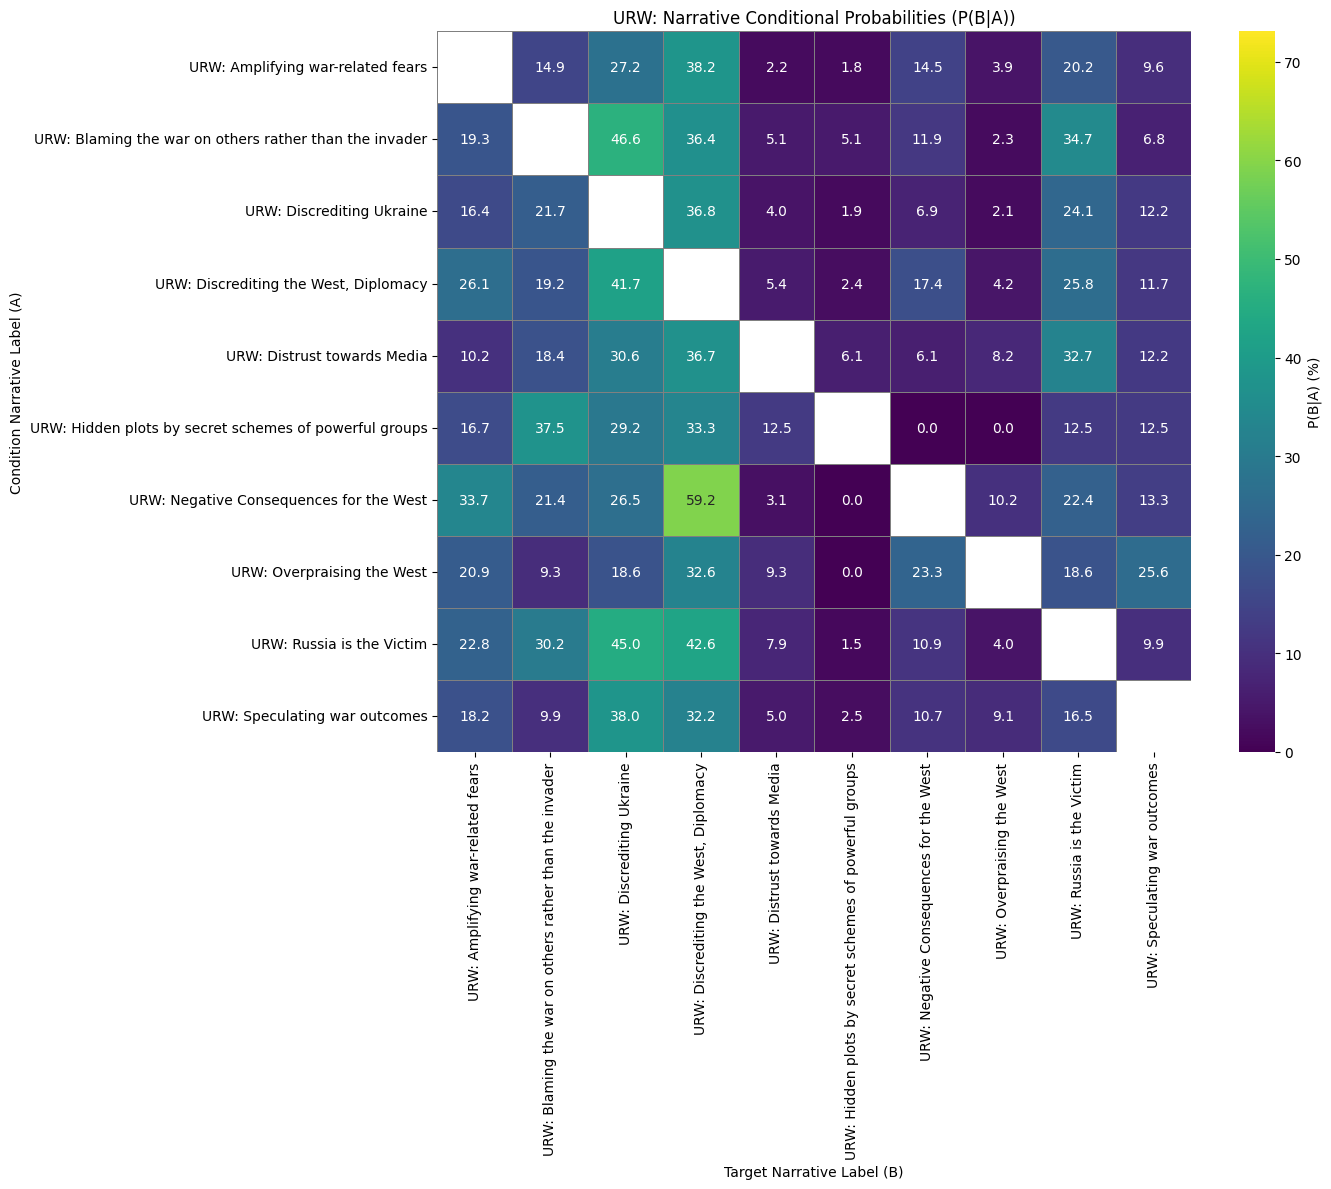
\includegraphics[width=\linewidth]{images/URW_narrative_conditional_probability.png}
  \par\medskip\centering\footnotesize (b) URW narratives conditional graph\par
  \end{minipage}
  \caption{Co-occurrence / conditional-probability visualizations for the most frequent narrative groups. (a) Heatmap for CC narratives (normalized cell values). (b) Heatmap for URW narratives. These paired views help identify both symmetric and directional dependencies among narratives.}
  \label{fig:narrative_cooccurrence}
\end{figure}

\textbf{Language-Specific Patterns.} These structural complexities are further nuanced by cross-lingual variations. The dataset exhibits notable variation across languages, with the average number of labels per document (label density) highest in Portuguese (\(\approx\) 3.04) and lower in Hindi (\(\approx\) 1.79), suggesting potential differences in source document complexity or annotation practices. Furthermore, the prevalence of specific narratives and their co-occurrence patterns differ across languages. This cross-lingual heterogeneity underscores the importance of using language-aware methods or, at a minimum, explicitly validating a model's performance on each language.

\textbf{Document Length Heterogeneity.} Finally, the dataset presents additional challenges through its variable document lengths. The corpus exhibits high variability, with a mean of approximately 404 words, a median of 371 words, and a range spanning from 45 to 4,422 words. This heterogeneity necessitates the use of effective truncation or long-text handling strategies in model design to manage computational constraints without losing critical context.